\hypertarget{methods}{%
	\section{Methods}\label{methods}}


\subsection*{Research Design}
This research study was accomplished under the Midwest Cooperative Ecosystems Study Unit (CESU). The CESU commissioned North Dakota State University to complete this work and respond to the objectives set forth in the Scope of Work. To accomplish these objectives fully, the NDSU research team applied a mixed method approach to fully understand management goals, current data gaps and desired outcomes for grassland management in these Midwest region NPS units. This approach included both qualitative and quantitative data collection methods. Interviews, surveys, and data audits collectively inform the recommendations communicated at the conclusion of this report. 
\subsection{Study Area}
The CESU Scope of Work named five NPS units spanning four states under the jurisdiction of the NPS Midwest Region office in Omaha, Nebraska (Fig. \ref{RegionMap}):
\begin{itemize}
\singlespacing
	\item Agate Fossil Beds National Monument (Nebraska) 
	\item Badlands National Park
(South Dakota) 
	\item Tallgrass Prairie National Preserve (Kansas)
	\item Theodore Roosevelt National Park (North Dakota)
	\item Wind Cave National Park (South Dakota)
\end{itemize}
	
 These NPS units all contain substantial grassland area,
although they are also geomorphologically and hydrologically variable \citep{gitzen2010}.

\begin{figure*}[th]
	\centering
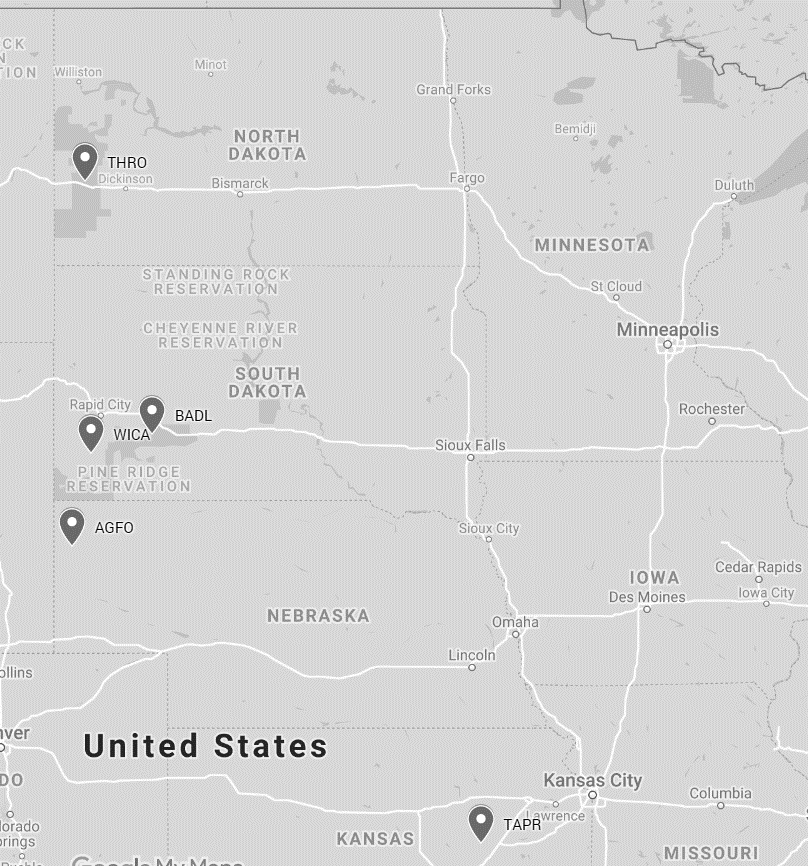
\includegraphics[width=0.75\textwidth]{figures/RegionMapGoogle.png}
\caption[Map of Midwest NPS units.]
	{Geographic location of NPS units included in this study.} 
\label{RegionMap}
\end{figure*}

Researchers visited the units in late spring 2018. 
Data audits and interviews of management staff were conducted at each site to understand management goals and availability of data.

\hypertarget{data-collection}{%
	\subsection{Data Collection}\label{data-collection}}

\subsubsection{Interviews and Surveys} 
Interviews were in-person and semi-structured. 
This format allowed us to cover certain topics in each
interview while allowing managers to discuss what they are passionate about \citep{creswell2003, montello2012}. 
Items in the interview guide are included as Appendix \ref{app:interview}. Interview questions were developed by using an established framework (Fig. \ref{LubellFramework}) created under previous social-ecological describing rangeland manager decision making \citep{lubell2013}. 
The framework focuses on factors influencing management decisions and how they evolve in response to dynamic social- ecological system characteristics.

\begin{figure*}[t]
	\begin{minipage}{0.3\textwidth}
		\raggedright
		\caption[Adaptive management frameworks]
		{A general and an NPS-specific framework for adaptive rangeland management. \\
		\emph{Top}: The general adaptive management decision-making framework from \citet{lubell2013}. \\
		\emph{Bottom}: An NPS-specific framework for adaptive management modified from the adaptive rangeland management decision-making framework by \citet{lubell2013}. \\
		Although not an explicit component of the analysis in this report, these frameworks helped us identify relevant topics to address in interviews and provided a means to contextualize responses. } \label{LubellFramework}
	\end{minipage}
\begin{minipage}{0.8\textwidth}
	\centering
	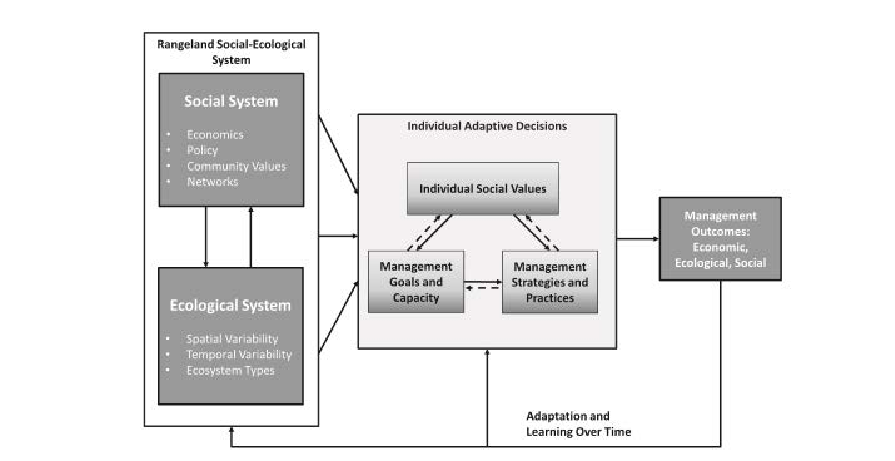
\includegraphics[width=0.75\textwidth]
		{figures/LubellFramework.pdf}

	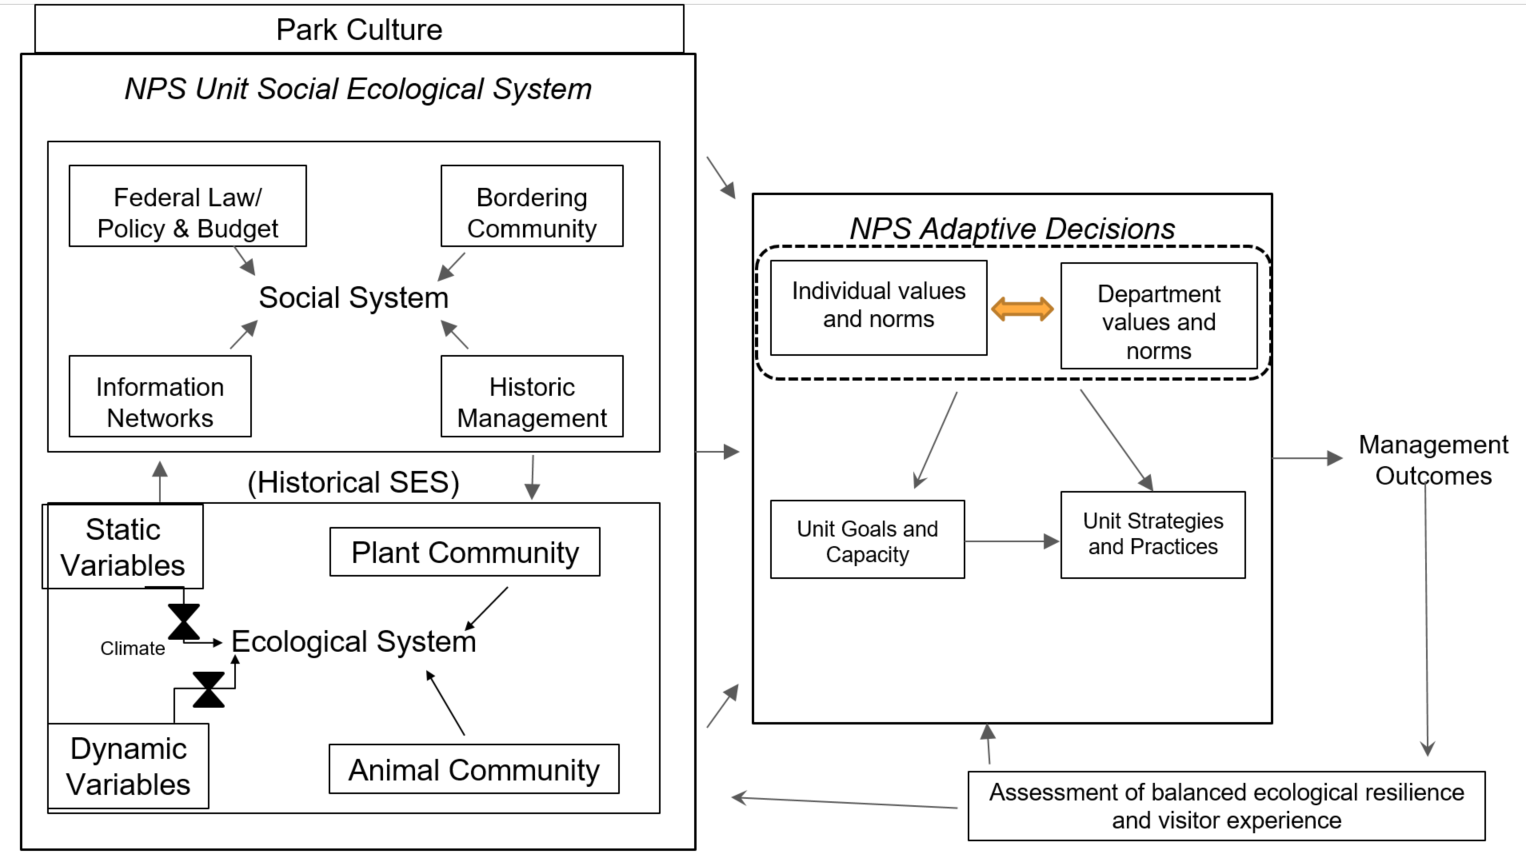
\includegraphics[width=0.75\textwidth]
		{figures/nps.png}
			\end{minipage}
\end{figure*}


We adapted the decision making framework to describe the process in terms of NPS decision making (Fig.~\ref{NPSframework}).
In early 2018, we attended a MWR Bison Strategic Meeting and conducted a focus group to aid in formation of the altered framework. 
The social system influencing decision making varies considerably between the two. 
NPS managers must take into account other opinions at their unit, visitor wants and needs, and budgetary constraints.

B. York conducted 18 interviews, recording them for later transcription.
Interviews were coded using the \sw{RQDA} package for Qualitative Analysis in the \R statistical environment  \citep{rcoreteam2017,huang2018} to identify common themes and inform the survey instrument.
Interviews helped us better understand sources of current uncertainties and overall management goals.

We created items on the survey to understand goals, management plans, data availability, and knowledge gaps in grassland management. 
We tailored the survey to inform the three objectives of this study. 
We sent out the survey with an invitation to participate and an invitation to disseminate the survey to others at their unit. 
It was developed in Google Forms and questions can be seen in Appendix \ref{app:survey}. 
We used responses to support to final management recommendations.

\subsubsection{Data Audits} 
Three sources of information informed data audits of each park service unit. 
Ahead of site visits, the Integrated Resource Management Applications (IRMA) portal provided a large amount of information. 
Researchers looked through publicly available data and management plans housed within IRMA. 
They also discussed data and management plans with unit staff that may have been not available to the public.

On-site visits revealed the second source of information. 
A search of file cabinets yielded paper copies of management plans, data files, and research studies conducted in the park. 
A researcher flagged topics related to grassland management and scanned these documents for later analysis at NDSU. 
This included but was not limited to: wildlife, vegetation, hydrology, geology, and fire. 
We also searched digital copies on NPS site servers in the same manner. Organization of files occurred once back at NDSU.

Finally, the data audit was completed with a literature review where we looked for academic studies accomplished in the units. 
We found studies conducted in the parks by using academic search engines as well as looking into Investigator Annual Reports (IAR) for each unit. 
The records found during the data audits can be seen in detail in the site specific appendices following this report.

